% Name: Scatter plot with a regression line
% Description: Exam scores against hours studied, with the least-squares line that pgfplots computes from the data and its equation in the legend.
% Tags: linear regression, least squares, scatter plot, trend line

\usepackage{pgfplots}
\usepackage{pgfplotstable}
\pgfplotsset{compat=1.18}

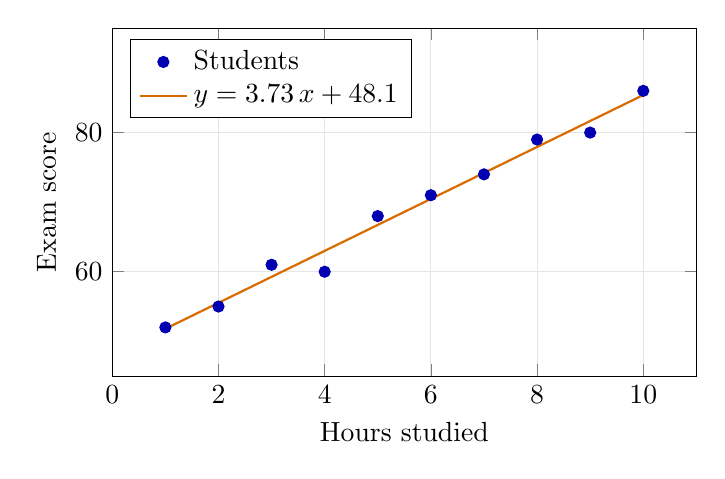
\begin{tikzpicture}
  \pgfplotstableread{
    hours score
    1     52
    2     55
    3     61
    4     60
    5     68
    6     71
    7     74
    8     79
    9     80
    10    86
  }\scores
  \begin{axis}[
    width=9cm, height=6cm, xmin=0, xmax=11, ymin=45, ymax=95,
    xlabel={Hours studied}, ylabel={Exam score},
    legend pos=north west, legend cell align=left,
    grid=major, grid style={gray!20},
  ]
    \addplot[only marks, mark=*, blue!70!black] table[x=hours, y=score] {\scores};
    \addlegendentry{Students}
    \addplot[thick, orange!85!black] table[x=hours, y={create col/linear regression={y=score}}] {\scores};
    \addlegendentry{$y = \pgfmathprintnumber[fixed, precision=2]{\pgfplotstableregressiona}\,x + \pgfmathprintnumber[fixed, precision=1]{\pgfplotstableregressionb}$}
  \end{axis}
\end{tikzpicture}
